\documentclass[11pt]{article}
\usepackage[a4paper,margin=24mm]{geometry}
\usepackage{amsmath,amssymb,amsthm}
\numberwithin{equation}{section}
\usepackage[T1]{fontenc}
\usepackage{lmodern}
\usepackage{tikz}
\usepackage{needspace}
\usepackage{array}
\newcolumntype{L}[1]{>{\raggedright\arraybackslash}p{#1}}
\AddToHook{cmd/subsection/before}{\ifnum\value{section}=3\Needspace{18\baselineskip}\fi}
\usepackage[hidelinks]{hyperref}
\newtheorem{theorem}{Theorem}[section]
\newtheorem{proposition}[theorem]{Proposition}
\newtheorem{corollary}[theorem]{Corollary}
\newtheorem{lemma}[theorem]{Lemma}
\theoremstyle{definition}
\newtheorem{definition}[theorem]{Definition}
\theoremstyle{plain}
\newcommand{\R}{\mathbb R}
\newcommand{\C}{\mathbb C}
\newcommand{\Sch}{\mathcal S(\R;\C)}
\newcommand{\diag}{\operatorname{diag}}
\newcommand{\Rea}{\operatorname{Re}}
% Vetting rounds: blue until accepted, then redefined as plain text with the date.
\newcommand{\reva}[1]{#1}
\newcommand{\revb}[1]{#1}
\newcommand{\revtag}[1]{#1}
\title{Gaussian states, covariance matrices and the formal Fock space}
\author{}
\date{}
% Navigation only; checked labels are maintained with reviewed correspondence.
\definecolor{GaussianTagFill}{HTML}{EEEAF8}
\definecolor{GaussianTagBorder}{HTML}{D6CEEB}
\definecolor{GaussianTagText}{HTML}{5B477D}
\newcommand{\BosonicLeanTag}{%
  \tikz[baseline=(tag.base)]\node[rounded corners=1.5pt,
    fill=GaussianTagFill,draw=GaussianTagBorder,text=GaussianTagText,
    line width=0.3pt,inner xsep=3pt,inner ysep=1.5pt] (tag)
    {\normalfont\scriptsize\sffamily Lean\,\ensuremath{\checkmark}};}
\makeatletter
\newcommand{\GaussianCheckedLabel}[1]{\expandafter\gdef\csname gaussian@checked@#1\endcsname{}}
\newcommand{\GaussianEnableLinks}{%
  \let\GaussianOriginalLabel\label
  \renewcommand{\label}[1]{%
    \GaussianOriginalLabel{##1}%
    \ifcsname gaussian@checked@##1\endcsname
      \nobreak\hspace{0.4em}\hyperlink{lean:##1}{\BosonicLeanTag}%
    \fi}}
\makeatother

\GaussianCheckedLabel{thm:congruence}
\GaussianCheckedLabel{thm:subsystem}
\GaussianCheckedLabel{thm:sum}
\GaussianCheckedLabel{prop:diagonal}
\GaussianCheckedLabel{thm:normalized}
\GaussianCheckedLabel{thm:moments}
\GaussianCheckedLabel{thm:covariance}
\GaussianCheckedLabel{cor:physical}
\GaussianCheckedLabel{thm:admissible-positive}
\GaussianCheckedLabel{thm:contraction}
\GaussianCheckedLabel{thm:periodic}
\GaussianCheckedLabel{prop:three-site}
\GaussianCheckedLabel{thm:fourier-contraction}
\GaussianCheckedLabel{thm:fourier-reconstruction}
\GaussianCheckedLabel{thm:periodic-product}
\GaussianCheckedLabel{cor:product-examples}

\GaussianCheckedLabel{thm:fock-ccr}
\GaussianCheckedLabel{lem:fock-raising}
\GaussianCheckedLabel{thm:fock-explaw}
\GaussianCheckedLabel{lem:fock-factorial}
\GaussianCheckedLabel{lem:fock-shift}
\GaussianCheckedLabel{thm:fock-bargmann}
\GaussianCheckedLabel{thm:fock-exp-bargmann}

\begin{document}
\GaussianEnableLinks
\maketitle
\vspace{-2em}
\noindent Gaussian formalism expresses properties of bosonic quantum states in terms
of phase-space data. For Gaussian states, the first moments and covariance matrix
determine the state: the former give its mean position and momentum, and the latter
describe its fluctuations. These notes develop the matrix algebra of covariances
and connect it with explicit normalized Gaussian wave functions, laying foundations
for the study of Gaussian matrix product states. For general background, see
Weedbrook et al.~\cite[Sec.~II]{weedbrook}.

\medskip
\enlargethispage{2\baselineskip}
\tableofcontents
\clearpage

\section*{About these notes}
\noindent These notes assume finite-dimensional linear algebra, complex inner products,
Lebesgue integration and elementary differential calculus. We begin with the matrix inequality governing admissibility,
then construct normalized Gaussian wave functions and compute their covariances.
\reva{Sections~\ref{sec:contraction}--\ref{sec:products} contract local covariances into
periodic Gaussian matrix product states.}

\medskip
\noindent\reva{Section~\ref{sec:fock} is of a different kind: it builds the formal Fock space
of all coefficient families over the number basis, the ladder operators on it, the
exponentials of operators that raise the photon number, and the Bargmann picture. It needs
only algebra and formal power series, and it is the foundation of the Gaussian-augmented
bosonic matrix product states of~\cite{tjoacirac}.} \revtag{These notes do not yet connect the
covariance matrices of Sections~1--5 with the formal Fock space.}

\medskip
\noindent\revtag{\textbf{Reading conventions.} The conventions of these notes are those of the
reading guide below, which compares each with the usual physics presentation.}

\medskip
\noindent\revtag{A statement marked
\BosonicLeanTag{} has a checked proof in BosonicLean whose correspondence with the statement
here has been reviewed; the declaration index at the end names the checked declarations. Definitions, Remarks and paragraphs of motivation carry no marks.}

\clearpage
% Reading guide.
\section*{Reading guide}
\addcontentsline{toc}{section}{Reading guide}
\noindent\revs{Where our objects or conventions differ from the usual physics presentation, the
table names the object used here, the one used in the literature, and where the two are related.}

\medskip
\noindent\revb{\begin{tabular}{@{}L{0.27\textwidth}L{0.31\textwidth}L{0.36\textwidth}@{}}
\textbf{Here} & \textbf{In the literature} & \textbf{Relation}\\[2pt]\hline\\[-8pt]
Covariance $\gamma$, twice the symmetrized covariance; vacuum $I_2$ &
Varies: vacuum $I_2$ as here (Weedbrook et al.~\cite{weedbrook}, quadratures $a+a^\dagger$);
$\sigma=\gamma/2$ with vacuum $\tfrac12I_2$ when $\sigma$ is the symmetrized covariance itself; or
$\hbar$-dependent units &
Definition~\ref{def:covariance}; units in Section~\ref{sec:states}\\[6pt]
Coordinates $(q_1,\ldots,q_n,p_1,\ldots,p_n)$, form $\Omega_n$ &
Mode by mode, $(q_1,p_1,\ldots,q_n,p_n)$ (e.g.~\cite{weedbrook}) &
A permutation of coordinates carries one symplectic form to the other; covariances transform by
the same permutation, by congruence, and admissibility is unchanged (proof of
Theorem~\ref{thm:sum})\\[6pt]
Admissibility $\gamma-i\Omega_n\succeq0$ &
Uncertainty relation for the covariance, e.g.\ $V+i\Omega\succeq0$ &
Definition~\ref{def:admissible}; equivalent to $\gamma+i\Omega_n\succeq0$ by complex conjugation,
and for $\sigma=\gamma/2$ to $\sigma-\tfrac i2\Omega_n\succeq0$\\[6pt]
Schwartz functions inside $L^2(\R)$ &
Wave functions &
Section~\ref{sec:states}\\[6pt]
Contraction: a Schur complement of covariance matrices &
Projection of virtual modes onto EPR pairs &
Section~\ref{sec:contraction}: the ideal EPR vector is not normalizable; the Schur complement is
proved, the EPR projection is its motivation\\[6pt]
Finite periodic chains, $N\ge3$ (translation-invariant in Section~\ref{sec:fourier}) &
Often infinite chains &
Sections~\ref{sec:contraction}--\ref{sec:products}\\[6pt]
Formal Fock space: all coefficient families &
The Hilbert space $\Gamma_s(\mathfrak h)$ &
$\Gamma_s(\mathfrak h)$ is the square-summable part (Section~\ref{sec:fock})\\[6pt]
$e^T$ as a finite sum at each coefficient, for $T$ raising the \revs{particle} number &
Operator exponential &
Equal coefficientwise wherever the series converges (after Lemma~\ref{lem:fock-raising})\\[6pt]
Bargmann map into formal power series &
Bargmann's space of entire functions &
On $\Gamma_s(\mathfrak h)$, the Taylor coefficients (after Definition~\ref{def:fock-bargmann})\\
\end{tabular}}

% Roadmap (lecture-form pass, 15 Oct 2026).
\section*{Roadmap}
\addcontentsline{toc}{section}{Roadmap}
\noindent\revs{Section~\ref{sec:covariance} characterizes covariance matrices by the matrix
inequality~\eqref{eq:admissibility} and proves that symplectic congruence, the selection of a
subsystem and independent sums preserve it. Section~\ref{sec:states} constructs normalized
Gaussian wave functions and computes their covariances, which realize the equality case of the
one-mode criterion of Proposition~\ref{prop:diagonal}. Section~\ref{sec:contraction} defines the
contraction of covariance matrices, a Schur complement motivated by EPR measurements on virtual
modes, proves that it preserves admissibility, and assembles from it the covariance of a periodic
Gaussian matrix product state. Sections~\ref{sec:fourier} and~\ref{sec:products} treat two cases
of that construction: chains with the same local covariance at every site, whose covariance splits into one
$2\times2$ block per frequency, and products.}

\medskip
\noindent\revs{Section~\ref{sec:fock} uses none of Sections~\ref{sec:covariance}--\ref{sec:products}.
From algebra and formal power series alone it builds the formal Fock space of all coefficient
families over the number basis, its ladder operators, the exponentials of operators that raise the
particle number, and the Bargmann picture; it is the foundation of the Gaussian-augmented bosonic
matrix product states of~\cite{tjoacirac}. Figure~\ref{fig:roadmap} shows which sections use
which.}

\begin{figure}[ht]
\centering
\revs{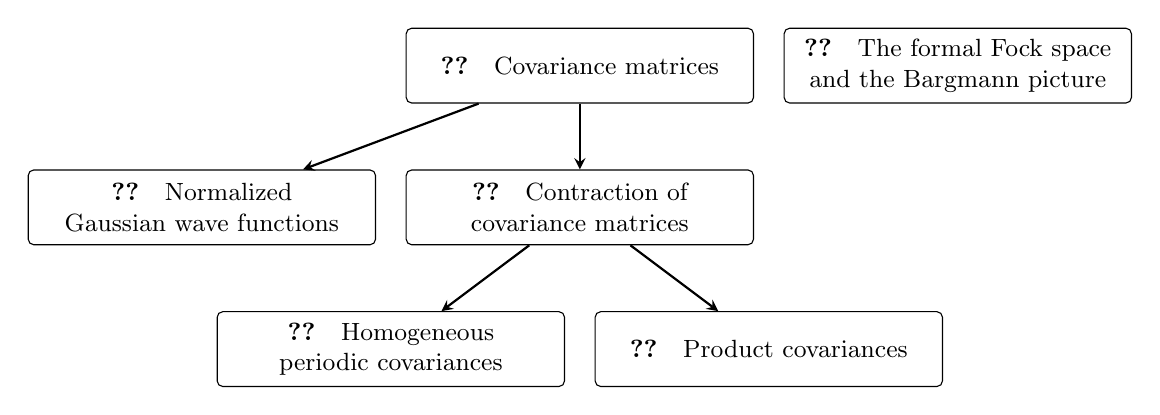
\begin{tikzpicture}[font=\small,
  sec/.style={draw, rounded corners=2pt, text width=4.2cm, align=center, minimum height=0.95cm,
    inner sep=3pt, execute at begin node={\hyphenpenalty=10000}},
  dep/.style={->, >=stealth, thick}]
  \node[sec] (s1) at (0,0) {\ref*{sec:covariance}\quad Covariance matrices};
  \node[sec] (s2) at (-4.8,-1.8) {\ref*{sec:states}\quad Normalized Gaussian wave functions};
  \node[sec] (s3) at (0,-1.8) {\ref*{sec:contraction}\quad Contraction of covariance matrices};
  \node[sec] (s4) at (-2.4,-3.6) {\ref*{sec:fourier}\quad Homogeneous periodic covariances};
  \node[sec] (s5) at (2.4,-3.6) {\ref*{sec:products}\quad Product covariances};
  \node[sec] (s6) at (4.8,0) {\ref*{sec:fock}\quad The formal Fock space and the Bargmann picture};
  \draw[dep] (s1) -- (s2);
  \draw[dep] (s1) -- (s3);
  \draw[dep] (s3) -- (s4);
  \draw[dep] (s3) -- (s5);
\end{tikzpicture}}
\caption{\revs{Dependence of the sections. An arrow means that the later section uses the earlier
one; arrows implied by a chain of arrows are omitted. Section~\ref{sec:states} enters
Sections~\ref{sec:contraction} and~\ref{sec:products} only in remarks, and Section~\ref{sec:fock}
uses no other section.}}
\label{fig:roadmap}
\end{figure}

\section{Covariance matrices}
\label{sec:covariance}
For $n\geq0$, use coordinates
$(q_1,\ldots,q_n,p_1,\ldots,p_n)$ on $\R^{2n}$ and define
\[
 \Omega_n=\begin{pmatrix}0&I_n\\-I_n&0\end{pmatrix}.
\]
For a complex matrix $H$, the notation $H\succeq0$ means that $H=H^*$ and
$z^*Hz\geq0$ for every complex column vector $z$. Here $H^*$ is the conjugate
transpose. Real matrices are regarded as complex matrices when used in this
inequality.

\begin{definition}[Admissible covariance]\label{def:admissible}
A real $2n\times2n$ matrix $\gamma$ is called \emph{admissible} if
\begin{equation}\label{eq:admissibility}
 \gamma^T=\gamma,\qquad \gamma-i\Omega_n\succeq0.
\end{equation}
\end{definition}
These coordinates are dimensionless. For one mode the condition concerns the
Hermitian matrix
\[
 \begin{pmatrix}a&c-i\\c+i&b\end{pmatrix},
 \qquad \gamma=\begin{pmatrix}a&c\\c&b\end{pmatrix}.
\]
The imaginary part records the canonical pairing between position and momentum.
The empty matrix is admissible when $n=0$.

\subsection{Changes of coordinates}
A real matrix $S$ is symplectic in these coordinates when
$S\Omega_nS^T=\Omega_n$. Transforming a covariance in both indices gives
$\gamma\mapsto S\gamma S^T$. This is a congruence transformation. Similarity
has the form $A\mapsto SAS^{-1}$; the two formulas agree for orthogonal $S$,
but symplecticity alone does not give $S^T=S^{-1}$.

\begin{theorem}\label{thm:congruence}
Let $n\geq0$ and let $S,\gamma$ be real $2n\times2n$ matrices. If $\gamma$
is admissible and $S\Omega_nS^T=\Omega_n$, then $S\gamma S^T$ is admissible.
\end{theorem}
\begin{proof}
Symmetry follows from $(S\gamma S^T)^T=S\gamma^TS^T=S\gamma S^T$.
Put $H=\gamma-i\Omega_n$. Since $S$ is real,
\[
 S\gamma S^T-i\Omega_n=S(\gamma-i\Omega_n)S^T=SHS^*.
\]
This matrix is Hermitian, and for every $z\in\C^{2n}$,
\[
 z^*SHS^*z=(S^*z)^*H(S^*z)\geq0.
\]
The same identities hold for empty matrices.
\end{proof}

\subsection{Subsystems and independent sums}
To select a subsystem, a position coordinate and its matching momentum
coordinate must be selected together. A \emph{one-to-one map}, also called an
\emph{injective map} or an \emph{injection}, is a map $e$ such that
$e(i)=e(j)$ implies $i=j$. Thus a one-to-one map
$e:\{1,\ldots,m\}\to\{1,\ldots,n\}$ selects distinct modes without
repetitions, in the order
\[
 (q_{e(1)},\ldots,q_{e(m)},p_{e(1)},\ldots,p_{e(m)}).
\]
Write $E(q_j)=q_{e(j)}$ and $E(p_j)=p_{e(j)}$. The selected covariance has
entries $\gamma'_{ab}=\gamma_{E(a),E(b)}$.

\begin{theorem}\label{thm:subsystem}
For all $m,n\geq0$, every such selection from an admissible $n$-mode covariance
is an admissible $m$-mode covariance. The empty selection is included.
\end{theorem}
\begin{proof}
Symmetry is inherited by restriction. The $qq$ and $pp$ blocks of $\Omega_n$
vanish, and its $qp$ and $pq$ entries are $\delta_{ij}$ and $-\delta_{ij}$.
Injectivity gives $\delta_{e(i),e(j)}=\delta_{ij}$, so restriction along $E$
sends $\Omega_n$ to $\Omega_m$.

Thus $H'=\gamma'-i\Omega_m$ is the selected principal submatrix of
$H=\gamma-i\Omega_n$. It is Hermitian. Extending a vector $z\in\C^{2m}$
by zero on the unselected coordinates gives $\widetilde z\in\C^{2n}$ and
\[
 z^*H'z=\widetilde z^{\,*}H\widetilde z\geq0.
\]
\end{proof}

Conversely, independent covariance blocks can be combined without cross terms.
\begin{definition}[Independent sum]\label{def:independent-sum}
For arbitrary real matrices $A$ and $B$ of sizes $2n\times2n$ and
$2m\times2m$, write their position/momentum blocks as $A_{qq},A_{qp},A_{pq},A_{pp}$
and similarly for $B$. Define
\begin{equation}\label{eq:independent-sum}
 A\boxplus B=
 \begin{pmatrix}
 A_{qq}&0&A_{qp}&0\\
 0&B_{qq}&0&B_{qp}\\
 A_{pq}&0&A_{pp}&0\\
 0&B_{pq}&0&B_{pp}
 \end{pmatrix}
\end{equation}
in the order $(q_A,q_B,p_A,p_B)$. This is $\diag(A,B)$ reordered from
$(q_A,p_A,q_B,p_B)$; the definition makes no symmetry assumption.
\end{definition}

\begin{theorem}\label{thm:sum}
For all $n,m\geq0$ and all real matrices $A,B$ of the stated sizes,
$A\boxplus B$ is admissible if and only if both $A$ and $B$ are admissible.
\end{theorem}
\begin{proof}
The same coordinate permutation sends $\diag(\Omega_n,\Omega_m)$ to
$\Omega_{n+m}$. Hence the uncertainty matrix of $A\boxplus B$ is the
corresponding permutation of $\diag(A-i\Omega_n,B-i\Omega_m)$.
When both blocks are admissible, symmetry is preserved and the quadratic
form is the sum of two nonnegative quadratic forms. Hermiticity is inherited
from the blocks. Conversely, restriction to either collection of matching
position/momentum coordinates recovers that block and its uncertainty matrix.
Theorem~\ref{thm:subsystem} applies. Empty blocks cause no exception.
\end{proof}

\subsection{One-mode diagonal matrices}
The diagonal case gives explicit examples and fixes the scale of the uncertainty
bound. Put $D(a,b)=\diag(a,b)$ in the order $(q,p)$.
\begin{proposition}\label{prop:diagonal}
For all $a,b\in\R$, the matrix $D(a,b)$ is admissible if and only if
$a>0$ and $ab\geq1$.
\end{proposition}
\begin{proof}
The uncertainty matrix is
$H=\left(\begin{smallmatrix}a&-i\\i&b\end{smallmatrix}\right)$.
If $H\succeq0$, the coordinate vectors give $a,b\geq0$. If $a=0$,
the vector $(b+1,-i)^T$ gives the negative value $-b-2$; hence $a>0$.
The vector $(i,a)^T$ then gives $0\leq a(ab-1)$, and therefore $ab\geq1$.

For the converse, suppose $a>0$ and $ab\geq1$. Write $z=x+iy$, $w=u+iv$.
The quadratic form is real and satisfies
\begin{align*}
 Q&=(\overline z,\overline w)H(z,w)^T
   =a(x^2+y^2)+b(u^2+v^2)+2(xv-yu),\\
 aQ&=(ax+v)^2+(ay-u)^2+(ab-1)(u^2+v^2)\geq0.
\end{align*}
Thus $Q\geq0$; Hermiticity of $H$ is immediate.
\end{proof}

In particular, $I_2=D(1,1)$ is admissible. More generally,
$D(t,t^{-1})$ is admissible for every $t>0$. Its two variances in our covariance
convention are $t/2$ and $1/(2t)$; their product is $1/4$.
By contrast, $cI_2$ with $0\leq c<1$ is a positive semidefinite real matrix
but is not admissible, since $c^2<1$.
Theorem~\ref{thm:sum} combines admissible one-mode blocks into larger matrices.
We now construct wave functions whose covariances give the one-mode equality case.

\section{Normalized Gaussian wave functions}
\label{sec:states}
\begin{definition}[Schwartz space]\label{def:schwartz}
Let $\mathcal D=\Sch$ be the Schwartz space: a smooth function $f$ belongs to
$\mathcal D$ when
\[
 \sup_{x\in\R}|x|^r|f^{(k)}(x)|<\infty
 \qquad (r,k\in\mathbb N_0).
\]
\end{definition}
We use Lebesgue measure and put $\mathcal H=L^2(\R;\C)$. Elements of $\mathcal H$ are equivalence classes of functions: two functions
represent the same element if they agree almost everywhere. Schwartz decay makes
every $f\in\mathcal D$ square-integrable. The usual inclusion
\[
 J:\mathcal D\longrightarrow\mathcal H,\qquad Jf=[f],
\]
sends a Schwartz function to its class. It is injective: continuous functions
that agree almost everywhere agree everywhere. We henceforth identify $f$ with $Jf$
when taking an $L^2$ norm or inner product, writing
\[
 \|f\|_2=\|Jf\|_{\mathcal H},\qquad
 \langle f,g\rangle=\int_\R\overline{f(x)}g(x)\,dx.
\]
The inner product is conjugate-linear in its first argument.

\begin{definition}[Normalized representative]\label{def:state}
A normalized state representative is a Schwartz function $f\in\mathcal D$
with $\|f\|_2=1$.
\end{definition}

For $\hbar>0$, position and momentum act on the common invariant domain
$\mathcal D$ by
\[
 (Xf)(x)=xf(x),\qquad (P_\hbar f)(x)=-i\hbar f'(x).
\]
Multiplication by $x$ and differentiation preserve Schwartz space. Their images
therefore have well-defined $L^2$ norms and inner products.

\begin{definition}[Means and covariance]\label{def:covariance}
For an operator
$A:\mathcal D\to\mathcal D$ and a normalized $f$, define
\[
 \mu_f(A)=\Rea\langle f,Af\rangle,\qquad
 u_f(A)=Af-\mu_f(A)f.
\]
For the ordered pair $(R_1,R_2)=(X,P_\hbar)$, the covariance is
\begin{equation}\label{eq:state-covariance}
 (\gamma_f)_{jk}=2\Rea\langle u_f(R_j),u_f(R_k)\rangle.
\end{equation}
\end{definition}
In particular, $(\gamma_f)_{jj}=2\|u_f(R_j)\|_2^2$ is twice the variance.

\subsection{Existence and normalization}
For a width $s>0$, we consider the positive real function
\begin{equation}\label{eq:gaussian}
 \psi_s(x)=\frac{1}{\sqrt{\sqrt\pi\,s}}
            \exp\left(-\frac{x^2}{2s^2}\right).
\end{equation}
\begin{theorem}\label{thm:normalized}
For every $s>0$, the function $\psi_s$ belongs to $\mathcal D$ and satisfies
$\|\psi_s\|_2=1$. It determines a unique normalized state representative
with the pointwise values in~\eqref{eq:gaussian}.
\end{theorem}
\begin{proof}
Put $\phi(x)=e^{-x^2/2}$. We define the \emph{Hermite polynomials} by
\[
 H_0(x)=1,\qquad H_{k+1}(x)=xH_k(x)-H_k'(x)\quad(k\geq0).
\]
The \emph{Hermite derivative identity} is
\[
 \phi^{(k)}(x)=(-1)^k H_k(x)\phi(x).
\]
It follows by induction from $\phi'=-x\phi$ and the product rule.
For every $r\geq0$, $|x|^r\phi(x)\to0$ as $|x|\to\infty$.
Continuity bounds this function globally. Expanding $H_k$ into monomials
then bounds $|x|^r|\phi^{(k)}(x)|$ for each $r,k$.
Dilation by $x\mapsto x/s$, inclusion of real values into $\C$, and
multiplication by a constant preserve Schwartz space, so $\psi_s\in\mathcal D$.

The Gaussian integral gives
\[
 \|\psi_s\|_2^2
 =\frac{1}{\sqrt\pi\,s}\int_\R e^{-x^2/s^2}\,dx
 =\frac{\sqrt\pi\,s}{\sqrt\pi\,s}=1.
\]
A function with the prescribed pointwise values is equal to $\psi_s$.
\end{proof}
The pointwise formula~\eqref{eq:gaussian} fixes the overall phase of $\psi_s$.

\subsection{Action and moments}
\begin{theorem}\label{thm:moments}
For every $s,\hbar>0$,
\begin{gather}
 P_\hbar\psi_s=\frac{i\hbar}{s^2}X\psi_s,
 \qquad \mu_{\psi_s}(X)=\mu_{\psi_s}(P_\hbar)=0,\label{eq:action}\\
 \|X\psi_s\|_2^2=\frac{s^2}{2},\qquad
 \|P_\hbar\psi_s\|_2^2=\frac{\hbar^2}{2s^2},\label{eq:seconds}\\
 \langle X\psi_s,P_\hbar\psi_s\rangle=\frac{i\hbar}{2}.
 \label{eq:cross}
\end{gather}
The first identity holds as an equality of Schwartz functions.
\end{theorem}
\begin{proof}
Differentiating~\eqref{eq:gaussian} yields $\psi_s'=-(x/s^2)\psi_s$ and hence
the momentum action. The integrand in
$\langle \psi_s,X\psi_s\rangle$ is odd and integrable, so this complex
inner product vanishes.

Set $A=\|X\psi_s\|_2^2$. With $\langle\cdot,\cdot\rangle_\R$
denoting the real part of the complex inner product, integration by parts gives
\begin{equation}\label{eq:ibp}
 1-\frac{A}{s^2}
 =\langle \psi_s,(X\psi_s)'\rangle_\R
 =-\langle \psi_s',X\psi_s\rangle_\R
 =\frac{A}{s^2}.
\end{equation}
The first equality uses $(X\psi_s)'=\psi_s+x\psi_s'$ and normalization.
Schwartz decay removes the boundary term, and the derivative formula gives
the last equality. Thus $A=s^2/2$.

Complex linearity in the second argument now gives
\[
 \langle \psi_s,P_\hbar\psi_s\rangle=0,\qquad
 \langle X\psi_s,P_\hbar\psi_s\rangle
 =\frac{i\hbar}{s^2}A=\frac{i\hbar}{2}.
\]
Finally, $\|P_\hbar\psi_s\|_2^2=(\hbar^2/s^4)A=\hbar^2/(2s^2)$.
\end{proof}

\subsection{Covariance and units}
\begin{theorem}\label{thm:covariance}
For every $s,\hbar>0$, the covariance of $\psi_s$ is
\[
 \gamma_{\psi_s}=\begin{pmatrix}s^2&0\\0&\hbar^2/s^2\end{pmatrix}.
\]
If $T=\diag(s^{-1},s/\hbar)$ and
$\widetilde\gamma=T\gamma_{\psi_s}T^T$, then $\widetilde\gamma=I_2$
and $\widetilde\gamma$ is admissible in the sense
of~\eqref{eq:admissibility}.
\end{theorem}
\begin{proof}
The means vanish, so the centered vectors in~\eqref{eq:state-covariance}
are $X\psi_s$ and $P_\hbar\psi_s$. Equations~\eqref{eq:seconds}
give the diagonal entries. The cross moment~\eqref{eq:cross} is purely
imaginary, as is its complex conjugate, so both off-diagonal entries vanish.
Diagonal multiplication gives $\widetilde\gamma=I_2$.
Proposition~\ref{prop:diagonal}, with $a=b=1$, proves admissibility.
\end{proof}

The matrix $T$ converts position and momentum to the dimensionless quantities
$X/s$ and $sP_\hbar/\hbar$. The covariance before this change of units retains
$\hbar$; we express the admissibility criterion of Section~\ref{sec:covariance}
in dimensionless coordinates. With $\hbar=1$ and $t=s^2$, the original covariance is
$D(t,t^{-1})$, realizing the diagonal equality cases above.

\begin{corollary}\label{cor:physical}
Let $m,\omega,\hbar>0$ and set $s=\sqrt{\hbar/(m\omega)}$. Then
\[
 \gamma_{\psi_s}=\diag\left(\frac{\hbar}{m\omega},\hbar m\omega\right).
\]
\end{corollary}
\begin{proof}
Positivity gives $s>0$ and $s^2=\hbar/(m\omega)$. Substitution into
Theorem~\ref{thm:covariance} gives the formula.
\end{proof}

\clearpage
\section{Contraction of covariance matrices}
\label{sec:contraction}
We now turn to constructing Gaussian matrix product states from local Gaussian
resources~\cite[Secs.~3 and~6]{schuch}. At each site, we distinguish \emph{physical
modes}, which form the final system, from auxiliary \emph{virtual modes}. Neighbouring
sites are joined by EPR measurements on their virtual modes, and we seek the
covariance of the physical modes conditioned on the measurement outcomes.
At the covariance level, this construction leads to a Schur complement.
We first establish the general matrix result, then explain EPR measurements
and apply it to a periodic chain.

\begin{theorem}\label{thm:admissible-positive}
Every admissible $2n\times2n$ covariance matrix is positive definite:
$x^T\gamma x>0$ for every nonzero $x\in\R^{2n}$.
\end{theorem}
\begin{proof}
Put $H=\gamma_{\C}-i\Omega_n$, where the subscript denotes entrywise inclusion
in $\C$. For real $x$, skew-symmetry gives $x^T\Omega_nx=0$, and hence
\[
 x^*Hx=x^T\gamma x\geq0.
\]
For a positive semidefinite Hermitian matrix, a vector has zero quadratic
form precisely when it lies in the kernel. Thus, if $x^T\gamma x=0$, then
$Hx=0$. Taking imaginary parts gives $\Omega_nx=0$. Since $\Omega_n^2=-I$,
we obtain $x=0$. The quadratic form is therefore strictly positive away from
zero. When $n=0$, there is no nonzero vector and the assertion is vacuous.
\end{proof}

\begin{definition}[Contracted covariance]\label{def:contraction}
Let $W$ be a real $(k+2m)\times2n$ matrix. For a real symmetric $2n\times2n$ matrix $\gamma$, write
\[
 V=W\gamma W^T=\begin{pmatrix}E&F\\F^T&G\end{pmatrix},
 \qquad E\in\R^{k\times k}.
\]
The first $k$ output coordinates are to be eliminated; the last $2m$ are
retained in position-then-momentum order. When $E$ is invertible, define
\[
 \gamma_{\mathrm{out}}=G-F^TE^{-1}F.
\]
This is the \emph{Schur complement} of $E$ in $V$. For $k=0$, it reduces to $G$.
\end{definition}
The eliminated coordinates need not form a canonical subsystem. The next
condition makes their symplectic pairings vanish, both among themselves and
with the retained coordinates.

\begin{theorem}\label{thm:contraction}
Let $n,m,k\geq0$ and let $\gamma$ be admissible. Suppose $W^T$ is one-to-one
and
\[
 W\Omega_nW^T=
 \begin{pmatrix}0_{k\times k}&0\\0&\Omega_m\end{pmatrix}.
\]
Then $E$ is positive definite, hence invertible, and
$\gamma_{\mathrm{out}}$ is admissible.
\end{theorem}
\begin{proof}
Theorem~\ref{thm:admissible-positive} and injectivity of $W^T$ give, for $y\ne0$,
\[
 y^TVy=(W^Ty)^T\gamma(W^Ty)>0.
\]
Thus $V$ and its principal block $E$ are positive definite. Congruence of the
input uncertainty matrix yields
\[
 Q=W_{\C}(\gamma_{\C}-i\Omega_n)W_{\C}^*
  =\begin{pmatrix}E_{\C}&F_{\C}\\F_{\C}^*&G_{\C}-i\Omega_m\end{pmatrix}
  \succeq0.
\]
For any complex vector $z$, choose the eliminated component to cancel the first
block row. Direct block multiplication gives
\[
 \begin{pmatrix}-E_{\C}^{-1}F_{\C}z\\z\end{pmatrix}^{\!*}
 Q\begin{pmatrix}-E_{\C}^{-1}F_{\C}z\\z\end{pmatrix}
 =z^*\bigl((G-F^TE^{-1}F)_{\C}-i\Omega_m\bigr)z\geq0.
\]
Here complexification commutes with the inverse of the invertible real matrix
$E$. The output is real symmetric because $E$ and $G$ are symmetric and
$(E^{-1})^T=E^{-1}$. Its uncertainty matrix is consequently Hermitian, so the
quadratic-form inequality proves admissibility. The argument includes empty
eliminated or retained coordinate sets.
\end{proof}

\subsection{EPR measurements and covariance contraction}
Two pairs of canonical quadratures admit the commuting combinations
\[
 X_-=q_A-q_B,\qquad P_+=p_A+p_B,\qquad
 [X_-,P_+]=[q_A,p_A]-[q_B,p_B]=0.
\]
An \emph{EPR measurement} is the joint measurement of these two observables.
Their exact joint eigenvectors are generalized eigenvectors: they do not belong
to the two-mode Hilbert space. In particular, the ideal EPR vector is not a
normalizable state. Finite squeezing gives normalizable approximations, but we
must not treat the infinitely squeezed vector as a density operator of trace one.
Giedke and Cirac~\cite[Secs.~III--IV]{giedke} develop the covariance description of
Gaussian measurements.

Reversing both quadratures of $B$ is a canonical phase rotation. It replaces the
preceding pair by
\begin{equation}\label{eq:epr-plus}
 Y_q=q_A+q_B,\qquad Y_p=p_A-p_B.
\end{equation}
We use this convention for the virtual pairs below. Put
$\Theta=\diag(I_M,-I_M)$ for $M$ such pairs. If we denote the remaining modes
by $C$, the matrix
\[
 L=\begin{pmatrix}I&\Theta&0\\0&0&I_C\end{pmatrix}
\]
maps the quadrature vector in $A,B,C$ order to $(Y,C)$.
The identity $\Theta\Omega_M\Theta^T=-\Omega_M$ gives
$L\Omega L^T=\diag(0,\Omega_C)$, as required in Theorem~\ref{thm:contraction}.

We now compute the corresponding characteristic function, including its
normalization. For a centered Gaussian with covariance $\gamma$, write
\[
 \chi(t)=\langle e^{it^TR}\rangle=\exp(-t^T\gamma t/4).
\]
The factor $1/4$ follows from our convention that $\gamma$ is twice the ordinary
covariance. Thus the joint characteristic function of $Y$ and the retained
quadratures is $\chi(L^T(u,z))$. In $A,B,C$ coordinates,
$L^T(u,z)=(u,\Theta u,z)$: this explains the momentum sign in the contraction
of characteristic-function variables. Write
\[
 L\gamma L^T=\begin{pmatrix}E&F\\F^T&G\end{pmatrix}.
\]
Conditioning on the zero outcome integrates out the Fourier variable $u$.
The quadratic expression in the exponent is
\begin{align*}
 u^TEu+2u^TFz+z^TGz
 &=(u+E^{-1}Fz)^TE(u+E^{-1}Fz)\\
 &\quad+z^T(G-F^TE^{-1}F)z.
\end{align*}
Since $E$ is positive definite, the Gaussian integral is finite. Dividing by
its value at $z=0$ leaves the characteristic function with covariance
$G-F^TE^{-1}F$. More generally, for means $d_Y,d_C$ and outcome $a$, the usual
Gaussian conditioning formula is
\begin{equation}\label{eq:conditional-mean}
 d_{C\mid a}=d_C+F^TE^{-1}(a-d_Y),\qquad
 \gamma_{C\mid a}=G-F^TE^{-1}F.
\end{equation}
The outcome changes the mean, but not the conditional covariance. We understand
conditioning here through the outcome density, not as an event of positive
probability at one exact value. These formulas give the measurement interpretation;
Theorem~\ref{thm:contraction} establishes the covariance inequality directly.

In the Choi--Jamio{\l}kowski construction, the resource associated with a map
is obtained formally by applying the map to one half of an ideal EPR pair.
EPR contraction with the other half represents feeding an input to the map.
This turns the \revs{construction of Gaussian matrix product states} into contractions of local resources, but
still involves ideal EPR measurements. Moreover, a channel representative obtained
from an infinitely squeezed pair need not be a finite covariance matrix: the
identity channel already illustrates the difficulty. The results below use
finite admissible local matrices. Schuch, Wolf and Cirac describe the resource
construction in Sections~3 and~6 of~\cite{schuch};
their Section 5 replaces infinitely entangled bonds by finite ones while moving
the infinite entanglement into the local maps.

\subsection{A periodic chain}
At each site $i\in\mathbb Z/N\mathbb Z$, we introduce $M$ left virtual modes $A_i$,
$M$ right virtual modes $B_i$, and one retained mode $C_i$.
The pair on each edge joins $B_{i-1}$ to $A_i$. We assume $N\geq3$ and $M\geq1$.
The integer $M$ counts the \emph{virtual modes per bond}. Each bosonic mode has
an infinite-dimensional Hilbert space, so even $M=1$ can support entanglement.
With no virtual modes, $M=0$, the virtual Hilbert space is one-dimensional;
this is the counterpart of bond dimension $D=1$ for a qudit MPS. We can also
represent product covariances with $M\geq1$ by adding unused virtual modes.
A bound on $M$ alone does not bound entanglement entropy: the squeezing must
also be controlled.

\begin{definition}[Periodic covariance]\label{def:periodic}
Put $d=2M+1$ and let $\Gamma_i$ be real $2d\times2d$ matrices. The local mode
order is $(A_{i,1},\ldots,A_{i,M},B_{i,1},\ldots,B_{i,M},C_i)$, with positions
preceding momenta. Define $\gamma_{\rm loc}$ on $Nd$ modes by
\[
 (\gamma_{\rm loc})_{(u,i,a),(v,j,b)}=
 \begin{cases}(\Gamma_i)_{(u,a),(v,b)},&i=j,\\0,&i\ne j,\end{cases}
 \qquad u,v\in\{q,p\}.
\]
Globally, positions precede momenta; within either group, sites precede local
modes. The real linear map $W:\R^{2Nd}\to\R^{2NM}\oplus\R^{2N}$ has eliminated
coordinates
\[
 (Wx)_{q,i,a}=x_{q,A_i,a}+x_{q,B_{i-1},a},\qquad
 (Wx)_{p,i,a}=x_{p,A_i,a}-x_{p,B_{i-1},a},
\]
and retained coordinates $(Wx)_{q,C_i}=x_{q,C_i}$ and
$(Wx)_{p,C_i}=x_{p,C_i}$. Each output group is in position-then-momentum order.
When its eliminated block is invertible, the \emph{periodic covariance} is
\[
 \gamma_{\rm per}=\mathrm{SC}_{\R^{2NM}}(W\gamma_{\rm loc}W^T),
\]
where $\mathrm{SC}$ denotes the Schur complement of Definition~\ref{def:contraction}.
\end{definition}
For comparison with~\revs{\cite{schuch}}, we group all $A$ coordinates together, then all $B$
and all $C$ coordinates. If $R$ shifts the site index to the right,
$(Rx)_i=x_{i-1}$, the same map is
\[
 W=\begin{pmatrix}I_A&R\Theta_B&0\\0&0&I_C\end{pmatrix}.
\]
The shift acts identically on positions and momenta and preserves each mode
label. This is the matrix in Section~6, Eq.~(3) of~\cite{schuch}.

\begin{theorem}\label{thm:periodic}
Suppose every $\Gamma_i$ is admissible. Then $W^T$ is injective,
\[
 W\Omega_{Nd}W^T=\diag(0_{2NM},\Omega_N),
\]
the eliminated block of $W\gamma_{\rm loc}W^T$ is positive definite, and
$\gamma_{\rm per}$ is admissible.
\end{theorem}
\begin{proof}
The independent sum of the local covariances is admissible by
Theorem~\ref{thm:sum}, iterated over the sites. Reordering its positions and
momenta together gives $\gamma_{\rm loc}$ and preserves the uncertainty inequality.
For an output vector $(y_q,y_p,z_q,z_p)$, the $A$ components of its image under
$W^T$ are $y_q,y_p$, and the $C$ components are $z_q,z_p$. Hence $W^T$ is injective.
Each eliminated position--momentum pairing has an $A$ contribution $+1$ and a
$B$ contribution $-1$. They cancel, including after the common cyclic shift.
Distinct mode pairs and all pairings with $C$ vanish. The retained pairings
form $\Omega_N$. Apply Theorem~\ref{thm:contraction}.
\end{proof}

\subsection{Three correlated sites}
\begin{proposition}\label{prop:three-site}
Take $N=3$, $M=1$, and at each site let
\[
 K=\begin{pmatrix}0&0&1\\0&0&1\\1&1&0\end{pmatrix},\qquad
 S=\begin{pmatrix}I_3&0\\K&I_3\end{pmatrix},\qquad \Gamma_i=SS^T.
\]
Then $S$ is symplectic, $\Gamma_i$ is admissible, and the periodic covariance is
\[
 \gamma_{\rm per}=\diag(Q,P),\qquad
 Q=\begin{pmatrix}3/5&1/5&1/5\\1/5&3/5&1/5\\1/5&1/5&3/5\end{pmatrix},\quad
 P=\begin{pmatrix}2&-1/2&-1/2\\-1/2&2&-1/2\\-1/2&-1/2&2\end{pmatrix}.
\]
It is admissible. In particular, distinct sites have position--position covariance
entry $1/5$ and momentum--momentum covariance entry $-1/2$.
\end{proposition}
\begin{proof}
Since $K=K^T$, direct multiplication gives $S\Omega_3S^T=\Omega_3$.
The covariance $I_6$ is an independent sum of three one-mode vacua, so
Theorem~\ref{thm:congruence} gives admissibility of $SS^T$.
Let $R$ be the three-site cyclic right shift and $U$ the $3\times3$ all-ones
matrix. Multiplying the local covariance blocks gives
\[
 E=\begin{pmatrix}2I&0\\0&4I-R-R^T\end{pmatrix},\quad
 F=\begin{pmatrix}0&I+R\\I-R&0\end{pmatrix},\quad
 G=\begin{pmatrix}I&0\\0&3I\end{pmatrix}.
\]
Here $R+R^T=U-I$ and $U^2=3U$. Consequently
\[
 (4I-R-R^T)^{-1}=(5I-U)^{-1}=\tfrac15 I+\tfrac1{10}U,
\]
as multiplication checks. Since $U(I-R)=0$, the two diagonal blocks of
the Schur complement are
\begin{align*}
 Q&=I-(I-R)^T(\tfrac15I+\tfrac1{10}U)(I-R)
   =\tfrac25I+\tfrac15U,\\
 P&=3I-\tfrac12(I+R)^T(I+R)=\tfrac52I-\tfrac12U.
\end{align*}
The off-diagonal blocks vanish. Theorem~\ref{thm:periodic} proves admissibility.
\end{proof}

For this example, $QP=I_3$, so the associated Gaussian state is pure. Its
single-site covariance is $\diag(3/5,2)$, with determinant $6/5>1$; the
single-site reduced state is therefore mixed. Thus the state is entangled
across every partition of one site from the other two. These deductions use
the Gaussian purity criterion~\cite[Secs.~II.C--D]{weedbrook}\revs{, which is cited, not
proved here; Proposition~\ref{prop:three-site} establishes the displayed covariance and its admissibility}.
\section{Homogeneous periodic covariances}\label{sec:fourier}
Suppose that every site in the periodic construction uses the same local
covariance $\Gamma$. A cyclic shift then leaves the construction unchanged.
The finite Fourier transform separates its spatial frequencies: at each
frequency, we obtain the covariance by eliminating only the local virtual
coordinates. This gives the finite-chain form of the Fourier calculation
in~\cite[Sec.~6]{schuch}.

Fix $N\geq3$ and $M\geq1$, with one physical mode at each site. We retain the
ordering and predecessor wiring of Section~\ref{sec:contraction}.
For the local block calculations, we group the coordinates as $(a,b,c)$, where
$a=(q_A,p_A)$, $b=(q_B,p_B)$ and $c=(q_C,p_C)$. Write
\[
 \Gamma=\begin{pmatrix}\Gamma_{vv}&\Gamma_{vC}\\
                         \Gamma_{Cv}&\Gamma_{CC}\end{pmatrix},
 \qquad v=(a,b),\qquad \Theta=\diag(I_M,-I_M).
\]
Thus the virtual block has size $4M\times4M$, the cross block has size
$4M\times2$, and the physical block has size $2\times2$.
All blocks are taken in the order $(a,b,c)$.

\begin{definition}[Fourier blocks]\label{def:fourier-blocks}
Label sites and frequencies by $0,\ldots,N-1$, with indices interpreted
modulo $N$. Set
\[
 \phi_k=\frac{2\pi k}{N},\qquad
 \widehat f_k=\frac1{\sqrt N}\sum_{j=0}^{N-1}e^{-\mathrm i\phi_kj}f_j,
 \qquad Z_k=\begin{pmatrix}I_{2M}&e^{-\mathrm i\phi_k}\Theta\end{pmatrix}.
\]
Define
\begin{equation}\label{eq:fourier-schur}
 E_k=Z_k\Gamma_{vv}Z_k^*,\qquad F_k=Z_k\Gamma_{vC},\qquad
 S_k=\Gamma_{CC}-F_k^*E_k^{-1}F_k,
\end{equation}
where $*$ denotes conjugate transpose. Invertibility of $E_k$ follows from
the next theorem.
\end{definition}
The eliminated coordinates are $y_j=a_j+\Theta b_{j-1}$. Substituting
$j=r+1$ in the Fourier sum gives
\[
 \widehat{(b_{j-1})}_k=e^{-\mathrm i\phi_k}\widehat b_k,
 \qquad \widehat y_k=Z_k\binom{\widehat a_k}{\widehat b_k}.
\]

\begin{theorem}[Fourier contraction]\label{thm:fourier-contraction}
Let $\Gamma$ be admissible and let $\gamma_{\rm per}$ be its homogeneous
periodic covariance. Each $E_k$ is Hermitian positive definite, and
\[
 (\gamma_{\rm per})_{\alpha,i+1;\,\beta,j+1}
   =(\gamma_{\rm per})_{\alpha i,\beta j}
 \qquad(\alpha,\beta\in\{q,p\}).
\]
Its Fourier transform is block diagonal:
\begin{equation}\label{eq:fourier-diagonal}
 \frac1N\sum_{i,j=0}^{N-1}e^{-\mathrm i\phi_ki}
 (\gamma_{\rm per})_{\alpha i,\beta j}e^{\mathrm i\phi_lj}
 =\begin{cases}(S_k)_{\alpha\beta},&k=l,\\0,&k\ne l.\end{cases}
\end{equation}
\end{theorem}
\begin{proof}
For $r$ coordinates at each site, define $T_k^{(r)}:\C^r\to\C^{Nr}$ by
$(T_k^{(r)}v)_j=e^{\mathrm i\phi_kj}v$. Character orthogonality gives
\[
 (T_l^{(r)})^*T_k^{(r)}=N\delta_{lk}I_r,\qquad
 \frac1N\sum_kT_k^{(r)}(T_k^{(r)})^*=I_{Nr}.
\]
The independent local covariance acts as $\Gamma$ on each such subspace.
The shift calculation above shows that the wiring acts there as
$L_k=\diag(Z_k,I_2)$. Its transpose acts as $L_k^*$, since the contribution
from a $B$ coordinate uses the successor site. Consequently the wired
covariance has local matrix
\[
 L_k\Gamma L_k^*=\begin{pmatrix}E_k&F_k\\F_k^*&\Gamma_{CC}\end{pmatrix}.
\]
Write its global blocks as $E,F,G$, as in the contraction theorem. In particular,
\[
 ET_k^{(2M)}=T_k^{(2M)}E_k,\qquad
 FT_k^{(2)}=T_k^{(2M)}F_k,\qquad
 GT_k^{(2)}=T_k^{(2)}\Gamma_{CC}.
\]
Theorem~\ref{thm:admissible-positive} gives $\Gamma\succ0$ over the reals.
For complex vectors, put $Q=\Gamma-\mathrm i\Omega$, with the symplectic
matrix $\Omega$ expressed in the same coordinate order. Both $Q$ and
$Q^T$ are positive semidefinite, so their average $\Gamma$ is positive
semidefinite as well. Since $\Gamma$ is nonsingular, it is positive definite.
Its virtual principal block is therefore positive definite. The map $Z_k^*$
is injective, since its first block is the identity, and hence
$E_k=Z_k\Gamma_{vv}Z_k^*\succ0$.
By Theorem~\ref{thm:periodic}, the global block $E$ is also positive definite.
The first mode identity therefore implies
$E^{-1}T_k^{(2M)}=T_k^{(2M)}E_k^{-1}$.
Taking the Schur complement yields
\[
 \gamma_{\rm per}T_k^{(2)}=T_k^{(2)}S_k.
\]
Multiplication by $(T_l^{(2)})^*$ and orthogonality prove
\eqref{eq:fourier-diagonal}. A cyclic shift acts by a scalar on each Fourier
subspace, so $\gamma_{\rm per}$ commutes with cyclic shifts and is
translation invariant.
\end{proof}

\begin{theorem}[Reconstruction and uncertainty]\label{thm:fourier-reconstruction}
Under the same assumptions,
\begin{equation}\label{eq:fourier-reconstruction}
 (\gamma_{\rm per})_{\alpha i,\beta j}
 =\frac1N\sum_{k=0}^{N-1}e^{\mathrm i\phi_k(i-j)}(S_k)_{\alpha\beta}.
\end{equation}
Moreover,
\[
 S_{-k}=\overline{S_k},\qquad
 S_k-\mathrm i\Omega_1\succeq0,\qquad
 \Omega_1=\begin{pmatrix}0&1\\-1&0\end{pmatrix},
\]
where $-k$ is interpreted modulo $N$ and the bar is entrywise conjugation.
\end{theorem}
\begin{proof}
Insert the Fourier resolution of the identity into
$\gamma_{\rm per}T_k^{(2)}=T_k^{(2)}S_k$ to obtain
\eqref{eq:fourier-reconstruction}. Since $\gamma_{\rm per}$ is real,
conjugating its Fourier transform replaces each frequency by its negative.
The diagonal blocks in~\eqref{eq:fourier-diagonal} therefore satisfy
$S_{-k}=\overline{S_k}$. Finally, Theorem~\ref{thm:periodic} gives
$\gamma_{\rm per}-\mathrm i\Omega_N\succeq0$. Its pullback along $T_k^{(2)}$ is
$N(S_k-\mathrm i\Omega_1)$: the position and momentum coordinates use the
same Fourier vectors, whose squared norm is $N$. Dividing by $N>0$ proves
the inequality.
\end{proof}
The matrices $S_k$ can have complex entries. Conjugate frequencies together
reconstruct the real covariance; the uncertainty inequality for an individual
frequency is an inequality of complex Hermitian matrices.

\section{Product covariances}
\label{sec:products}
The periodic construction includes products: if the physical mode at each site
is independent of the virtual modes, contraction leaves its covariance unchanged.
We make this explicit, allowing the physical covariance to vary from site to site.
We retain $N\geq3$, $M\geq1$ and the ordering of Section~\ref{sec:contraction}.

\begin{definition}\label{def:product-resource}
Let $\eta_i$ be a real one-mode covariance at site $i$. Take the local covariance
\[
 \Gamma_i=\diag(I_{2M},I_{2M},\eta_i)
\]
in grouped phase coordinates $(q_{A_i},p_{A_i},q_{B_i},p_{B_i},q_{C_i},p_{C_i})$,
then reorder it to the position-then-momentum coordinates used for periodic
assembly. Define the physical product covariance by
\[
 (\gamma_{\rm prod})_{(u,i),(v,j)}=
 \begin{cases}(\eta_i)_{uv},&i=j,\\0,&i\ne j,\end{cases}
 \qquad u,v\in\{q,p\}.
\]
\end{definition}
Each virtual mode is a vacuum and is independent of all other modes at its site.
The physical mode has covariance $\eta_i$.

\begin{theorem}\label{thm:periodic-product}
If every $\eta_i$ is admissible, then every $\Gamma_i$ is admissible and
\[
 W\gamma_{\rm loc}W^T=
 \begin{pmatrix}2I_{2NM}&0\\0&\gamma_{\rm prod}\end{pmatrix}.
\]
Consequently the periodic contraction equals $\gamma_{\rm prod}$ and is
admissible. In particular, one virtual mode per bond suffices for every $N\geq3$.
\end{theorem}
\begin{proof}
The independent-sum rule of Theorem~\ref{thm:sum} applies to the local resources.
In grouped phase coordinates its uncertainty matrix is
\[
 \Gamma_i-i\diag(\Omega_M,\Omega_M,\Omega_1)
 = (I_{2M}-i\Omega_M)\oplus(I_{2M}-i\Omega_M)
       \oplus(\eta_i-i\Omega_1)\succeq0.
\]
The two vacuum blocks and the prescribed physical block are positive semidefinite;
reordering the coordinates preserves the inequality.

Each eliminated quadrature is the signed sum of two independent virtual vacuum
coordinates. Its diagonal covariance entry is $1+1=2$. Distinct eliminated
coordinates have zero covariance: distinct virtual modes are independent, and
within each vacuum mode the position--momentum covariance vanishes. The virtual
coordinates are also independent of every physical coordinate. Thus, in the
notation of Definition~\ref{def:contraction},
\[
 E=2I_{2NM},\qquad F=0,\qquad G=\gamma_{\rm prod}.
\]
The Schur-complement formula therefore gives
\[
 \gamma_{\rm per}=G-F^TE^{-1}F=\gamma_{\rm prod}.
\]
Admissibility follows from Theorem~\ref{thm:periodic}.
\end{proof}

\begin{corollary}\label{cor:product-examples}
For $\eta_i=I_2$ at every site, the periodic contraction is $I_{2N}$.
For arbitrary $s_i>0$, the choices
$\eta_i=\diag(s_i^2,s_i^{-2})$ give the corresponding product of squeezed
one-mode covariances.
\end{corollary}
\begin{proof}
The vacuum covariance is admissible. The diagonal criterion of
Proposition~\ref{prop:diagonal} states
\[
 \diag(a,b)\text{ is admissible}\quad\Longleftrightarrow\quad a>0\ \text{and}\ ab\geq1.
\]
Apply it with $a=s_i^2$ and $b=s_i^{-2}$, whose product is one, and use
Theorem~\ref{thm:periodic-product}. In the vacuum case, the entries of
$\gamma_{\rm prod}$ are those of the identity.
\end{proof}
The one-mode Gaussians of Theorem~\ref{thm:covariance}, with $\hbar=1$, have
these squeezed covariances. The virtual vacua in this construction are unused;
adding them allows products to fit the same $M\geq1$ convention as the correlated
examples.
% Formal Fock space, ladder operators, raising exponentials and the Bargmann picture.
% The bosonic matrix product states built on it: Tjoa and Cirac, arXiv:2607.28753.
\providecommand{\ket}[1]{\lvert #1\rangle}
\providecommand{\bra}[1]{\langle #1\rvert}
\providecommand{\Tr}{\operatorname{Tr}}
\providecommand{\N}{\mathbb N}
\providecommand{\Fock}{\mathcal F}
\providecommand{\Barg}{\mathfrak B}
\providecommand{\coef}[2]{[z^{#1}]\,#2}
\clearpage
\section{The formal Fock space and the Bargmann picture}\label{sec:fock}
The number basis of a bosonic Fock space labels vectors by occupation numbers. Allowing all
coefficient families, with no summability condition, gives a space on which the creation
operators and the exponentials of operators that raise the particle number act exactly, one
coefficient at a time. This section develops that formal Fock space, the canonical
commutation relations on it, the exponential law for raising operators, and the Bargmann
picture, in which creation and annihilation become multiplication by and differentiation in
formal variables. The exponentials of the Gaussian-augmented bosonic matrix product states of
Tjoa and Cirac~\cite{tjoacirac} are of this kind. \reva{Those states are a
different construction from the Gaussian matrix product states whose covariance matrices are
built by contraction in Sections~\ref{sec:contraction}--\ref{sec:products}; these notes do not
yet relate the two.}

\medskip
\noindent\textbf{Notation for this section.}
\begin{center}
\begin{tabular}{ll}
$\iota$ & a set of modes\\
$n=(n_i)_{i\in\iota}$ & a multi-index of occupation numbers, finitely many nonzero\\
$m$ & an occupation number of a single mode\\
$e_i$ & the multi-index with a single $1$ at $i$\\
$\lvert n\rvert=\sum_i n_i$ & total particle number of $n$\\
$n!=\prod_i n_i!$ & factorial of a multi-index\\
$\ket n$ & number state (Definition~\ref{def:fock-space})\\
$\Fock(\iota,R)$ & formal Fock space with coefficients in $R$ (Definition~\ref{def:fock-space})\\
$\mathfrak h$, $\Gamma_s(\mathfrak h)$ & for finite $\iota$, the one-particle space $\C^\iota$ and its Fock space\\
$a_i^\dagger,\ a_i$ & creation and annihilation operators (Definition~\ref{def:fock-ladder})\\
$T$, $T'$, $e^T$ & raising operators and their exponential (Definition~\ref{def:fock-raising})\\
$R[[z]]$, $\partial_j$ & formal power series in $(z_i)_{i\in\iota}$ over $R$; partial derivative\\
$\coef nf$ & coefficient of $z^n=\prod_iz_i^{n_i}$ in $f\in R[[z]]$\\
$\Barg$ & Bargmann map (Definition~\ref{def:fock-bargmann})\\
\end{tabular}
\end{center}
\reva{In this section $R$ is a $\C$-algebra, $X\in R$, $n$ a multi-index, $W$ a word in the
ladder operators, $T$ a raising operator, $p\ge1$ an exponent, $z$ the formal variables and
$\Lambda$ a bound on particle numbers; letters shared with
Sections~\ref{sec:covariance}--\ref{sec:products} do not carry their meanings from there.}

\subsection{The formal Fock space}

Throughout, $R$ is a $\C$-algebra: a ring together with a ring homomorphism from $\C$ into
its centre. The two cases used later are $R=\C$ (states) and $R=M_\beta(\C)$, the complex
matrices indexed by a finite set $\beta$ (vectors that carry a matrix index); for $\beta$
empty, $M_\beta(\C)$ is the zero ring, which is allowed.

\begin{definition}[Formal Fock space]\label{def:fock-space}
$\Fock(\iota,R)$ is the set of all functions $\psi$ from multi-indices to $R$, with
pointwise addition and scalar multiplication; $\psi$ is read as $\sum_n\psi(n)\ket n$.
The number state $c\ket n$ has coefficient $c$ at $n$ and $0$ elsewhere, and $\ket0$ is
the vacuum. A vector $\psi$ \emph{vanishes below $k$} if $\psi(n)=0$ whenever
$\lvert n\rvert<k$.
\end{definition}

No summability is imposed. For finite $\iota$ and the one-particle space $\mathfrak
h=\C^\iota$ with its standard orthonormal basis, the $k$-particle space
$\otimes_s^k\mathfrak h$ has as orthonormal basis the number states $\ket n$ with
$\lvert n\rvert=k$, so that, sector by sector,
\[
 \Gamma_{\mathrm{fin}}(\mathfrak h)=\bigoplus_{k}\otimes_s^k\mathfrak h\ \subset\
 \Gamma_s(\mathfrak h)=\overline{\bigoplus_{k}}\,\otimes_s^k\mathfrak h\ \subset\
 \prod_{k}\otimes_s^k\mathfrak h=\Fock(\iota,\C):
\]
the finite-particle space, the bosonic Fock space of~\cite{dg,br} (the Hilbert direct sum,
that is, the square-summable families) and the full product. \reva{$\Gamma_s(\mathfrak h)$
is recalled from~\cite{dg,br}; it is not constructed in these notes}\revs{, nor are second
quantization, the Fock representation of the CCR algebra, or the identification of
$\Gamma_s(\mathfrak h)$ with $L^2(\R^\iota)$ through the Hermite functions that would join this
section to Sections~\ref{sec:covariance}--\ref{sec:products}}. For a single mode, the vector with
coefficients $\sqrt{(2k)!}/k!$ at $\ket{2k}$ and $0$ at odd occupations lies in
$\Fock(\{1\},\C)$ but not in $\Gamma_s$, since $(2k)!/(k!)^2\ge1$. After
Definition~\ref{def:fock-raising} it is $e^{(a^\dagger)^2}\ket0$.

\begin{definition}[Ladder operators and left multiplication]\label{def:fock-ladder}
For $i\in\iota$, the creation and annihilation operators are the $\C$-linear maps
\[
 (a_i^\dagger\psi)(n)=\begin{cases}\sqrt{n_i}\,\psi(n-e_i),&n_i\ge1,\\0,&n_i=0,\end{cases}
 \qquad (a_i\psi)(n)=\sqrt{n_i+1}\,\psi(n+e_i).
\]
For $X\in R$, $X\psi$ is the vector with coefficients $X\psi(n)$. For a word $W$ in the
ladder operators, $X\otimes W$ denotes the composite $XW$; the two factors commute, since a
ladder word multiplies each coefficient by complex scalars and moves it, while $X$
multiplies it on the left, and complex scalars are central in $R$.
\end{definition}

On number states these are the formulas $a_i^\dagger\ket n=\sqrt{n_i+1}\ket{n+e_i}$ and
$a_i\ket n=\sqrt{n_i}\ket{n-e_i}$. On $\Gamma_s(\mathfrak h)$ the creation and annihilation
operators of~\cite{dg} are $a^*(h)=\sum_ih_ia_i^\dagger$ and $a(h)=\sum_i\overline{h_i}\,a_i$
for $h\in\mathfrak h$. Each coefficient of $a_i^\dagger\psi$ or $a_i\psi$ involves a single
coefficient of $\psi$, so both operators are defined on the whole formal Fock space.

\begin{theorem}[Canonical commutation relations]\label{thm:fock-ccr}
On all of $\Fock(\iota,R)$: $[a_i,a_j^\dagger]=\delta_{ij}$, $[a_i,a_j]=0$ and
$[a_i^\dagger,a_j^\dagger]=0$.
\end{theorem}

\begin{proof}
We check the identities coefficientwise.
\begin{enumerate}
\item[(a)] For $i=j$: $(a_ia_i^\dagger\psi)(n)=\sqrt{n_i+1}\sqrt{n_i+1}\,\psi(n)$ and
$(a_i^\dagger a_i\psi)(n)=\sqrt{n_i}\sqrt{n_i}\,\psi(n)$, the second being $0$ when $n_i=0$.
The difference is $\psi(n)$.
\item[(b)] For $i\ne j$, both orders give $\sqrt{n_j}\sqrt{n_i+1}\,\psi(n+e_i-e_j)$ when
$n_j\ge1$, and $0$ otherwise, because shifting $n_i$ does not change $n_j$.
\item[(c)] For $i\ne j$, $a_ia_j$ and $a_ja_i$ both multiply $\psi(n+e_i+e_j)$ by
$\sqrt{n_i+1}\sqrt{n_j+1}$; $a_i^\dagger a_j^\dagger$ and $a_j^\dagger a_i^\dagger$ both
multiply $\psi(n-e_i-e_j)$ by $\sqrt{n_i}\sqrt{n_j}$ when $n_i,n_j\ge1$, and give $0$
otherwise. For $i=j$ there is nothing to prove.\qedhere
\end{enumerate}
\end{proof}

\reva{Since $a_i^\dagger(c\ket n)=\sqrt{n_i+1}\,c\ket{n+e_i}$ and the creation operators
commute, $\prod_i(a_i^\dagger)^{n_i}(c\ket0)=\sqrt{n!}\,c\ket n$, the product running over the
finitely many $i$ with $n_i\ne0$. So $\ket n=\prod_i(a_i^\dagger)^{n_i}\ket0/\sqrt{n!}$, as
usual.}

\subsection{Raising operators and their exponentials}

Operators that raise the particle number have exponential series that are finite at each
coefficient.

\begin{definition}[Raising operator and its exponential]\label{def:fock-raising}
A $\C$-linear map $T$ on $\Fock(\iota,R)$ is \emph{raising} (short for order-raising) if, for
every $k$, $T\psi$
vanishes below $k+1$ whenever $\psi$ vanishes below $k$. For raising $T$,
\[
 (e^T\psi)(n)=\sum_{r=0}^{\lvert n\rvert}\frac{(T^r\psi)(n)}{r!}.
\]
\end{definition}

\begin{lemma}\label{lem:fock-raising}
Let $T$ and $T'$ be raising.
\begin{enumerate}
\item[(a)] If $T_1,\ldots,T_r$ are raising and $\psi$ vanishes below $k$, then
$T_1\cdots T_r\psi$ vanishes below $k+r$. In particular $(T^r\psi)(n)=0$ for
$r>\lvert n\rvert$, and $(e^T\psi)(n)=\sum_{r=0}^{\Lambda}(T^r\psi)(n)/r!$ for every
$\Lambda\ge\lvert n\rvert$.
\item[(b)] $(T\psi)(n)$ depends only on the coefficients $\psi(n')$ with
$\lvert n'\rvert<\lvert n\rvert$.
\item[(c)] $T+T'$, $TT'$ and $cT$ ($c\in\C$) are raising; so are $a_i^\dagger$ and, for
$X\in R$ and $p\ge1$, $X(a_i^\dagger)^p$.
\end{enumerate}
\end{lemma}

\begin{proof}
\begin{enumerate}
\item[(a)] Apply the definition to $T_r$, then $T_{r-1}$, and so on; each step raises the
bound by one. Every $\psi$ vanishes below $0$.
\item[(b)] If $\psi$ and $\psi'$ agree in degrees below $\lvert n\rvert$, then $\psi-\psi'$
vanishes below $\lvert n\rvert$, so $T(\psi-\psi')$ vanishes below $\lvert n\rvert+1$, in
particular at $n$.
\item[(c)] The first three claims follow from the definition. $(a_i^\dagger\psi)(n)$ is a
multiple of $\psi(n-e_i)$ and $\lvert n-e_i\rvert=\lvert n\rvert-1$, so $a_i^\dagger$ is
raising; hence so is $(a_i^\dagger)^p$ for $p\ge1$, and left multiplication by $X$
preserves vanishing below $k$.\qedhere
\end{enumerate}
\end{proof}

\reva{We define the exponential by the finite sum of Definition~\ref{def:fock-raising},
not as a limit, so no topology on $\Fock(\iota,R)$ is needed.} By Lemma~\ref{lem:fock-raising}(a) this is the operator series
$\sum_rT^r/r!$ itself: at every coefficient the partial sums are constant from
$r=\lvert n\rvert$ on. When the series converges in $\Gamma_s(\mathfrak h)$, its limit has
these coefficients, since convergence there implies convergence of each coefficient.

\begin{figure}[ht]
\centering
\revb{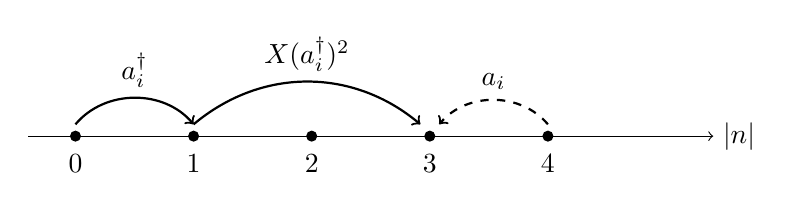
\begin{tikzpicture}[x=1.5cm]
 \draw[->] (-0.4,0) -- (5.4,0) node[right] {$\lvert n\rvert$};
 \foreach \k in {0,...,4} \fill (\k,0) circle (2pt) node[below=3pt] {$\k$};
 \draw[->,thick] (0,0.15) to[bend left=50] node[above] {$a_i^\dagger$} (1,0.15);
 \draw[->,thick] (1,0.15) to[bend left=40] node[above] {$X(a_i^\dagger)^2$} (2.92,0.15);
 \draw[->,thick,dashed] (4,0.15) to[bend right=50] node[above] {$a_i$} (3.08,0.15);
\end{tikzpicture}
\caption{Raising maps (solid) move every coefficient to strictly higher particle number; the
annihilation operator (dashed) moves it down. Hence the coefficient of $e^T\psi$ at particle
number $k$ receives only the terms $T^r\psi$ with $r\le k$: the finite sum of
Definition~\ref{def:fock-raising}.}\label{fig:fock-grading}}
\end{figure}

\begin{theorem}[Exponential law]\label{thm:fock-explaw}
If $T$ and $T'$ are raising and $TT'=T'T$, then $e^{T+T'}=e^Te^{T'}$.
\end{theorem}

\begin{proof}
\reva{By Lemma~\ref{lem:fock-raising}(c), $T+T'$ is raising, so both sides are
defined; likewise $T^r$ is raising for $r\ge1$, which is used below.} The coefficient of $e^Te^{T'}\psi$ at
$n$ reduces to a finite double sum, which the binomial theorem collapses. Fix $n$ and $\psi$,
and put $\Lambda=\lvert n\rvert$. By Lemma~\ref{lem:fock-raising}(a), $e^{T'}\psi$ agrees in all
degrees $\le\Lambda$ with $\sum_{t=0}^\Lambda T'^t\psi/t!$. By Lemma~\ref{lem:fock-raising}(b),
applied to the raising map $T^r$ for $r\ge1$ (and trivially for $r=0$),
\[
 (e^Te^{T'}\psi)(n)=\sum_{r=0}^\Lambda\sum_{t=0}^\Lambda\frac{(T^rT'^t\psi)(n)}{r!\,t!}
 =\sum_{k=0}^\Lambda\frac1{k!}\sum_{r+t=k}\binom kr(T^rT'^t\psi)(n)
 =\sum_{k=0}^\Lambda\frac{((T+T')^k\psi)(n)}{k!}.
\]
We dropped the terms with $r+t>\Lambda$ because $T^rT'^t$ is a product of $r+t$ raising maps and
therefore, by Lemma~\ref{lem:fock-raising}(a), vanishes at $n$; the last step is the
binomial theorem for commuting $T$ and $T'$. The right side is $(e^{T+T'}\psi)(n)$.
\end{proof}

For matrices the same identity rests on absolute convergence of the double series. Here the
grading by particle number replaces it. \reva{Without the raising hypothesis the finite sum of
Definition~\ref{def:fock-raising} need not agree with the series $\sum_r(T^r\psi)(n)/r!$, and
the series need not converge. For the annihilation operator $a$ of a single mode and
$\psi=\ket1$, the finite sum at $n=0$ is $\psi(0)=0$, while the series gives
$(a\psi)(0)=1$. For $\psi(m)=m!$, the series $\sum_k(a^k\psi)(0)/k!=\sum_k\sqrt{k!}$
diverges.}

\subsection{The Bargmann picture}

\reva{$R[[z]]$ is the set of all functions $f$ from multi-indices to $R$, written
$f=\sum_n\coef nf\,z^n$, with the Cauchy product
$\coef n{(fg)}=\sum_{n'+n''=n}\coef{n'}f\,\coef{n''}g$, a finite sum.} For $f\in R[[z]]$, we define the partial derivative coefficientwise by
$\coef n{(\partial_jf)}=(n_j+1)\,\coef{n+e_j}f$; for $R=\C$ it is the usual derivative of
formal power series.

\begin{definition}[Bargmann map]\label{def:fock-bargmann}
$\Barg:\Fock(\iota,R)\to R[[z]]$ is given by $\coef n{\Barg\psi}=\psi(n)/\sqrt{n!}$.
It is a $\C$-linear bijection, with inverse $\psi(n)=\sqrt{n!}\,\coef nf$.
\end{definition}

Thus $\Barg\ket n=z^n/\sqrt{n!}$, which for finite $\iota$ is the orthonormal basis of
Bargmann's space of entire functions~\cite{bargmann}. So $\Barg$ maps $\Gamma_s(\mathfrak h)$
onto the Taylor series of the Bargmann space, and the formal Fock space onto all of $R[[z]]$,
including, \reva{for a single mode and $R=\C$,} series such as $\sum_mm!\,z^m=\Barg\psi$,
$\psi(m)=m!\sqrt{m!}$, with radius of convergence $0$. A vector $\psi$ vanishes below $k$
exactly when $\Barg\psi$ has order at least $k$ (no monomial of total degree below $k$), so a
raising map raises the order of power
series by at least one; hence the name.

\begin{lemma}\label{lem:fock-factorial}
If $n_j\ge1$, then $n!=n_j\,(n-e_j)!$.
\end{lemma}

\begin{proof}
$n$ and $n-e_j$ differ only in the $j$-th entry, and $n_j!=n_j\,(n_j-1)!$.
\end{proof}

\begin{lemma}\label{lem:fock-shift}
For every $f\in R[[z]]$: $\coef n{(z_j^mf)}=\coef{n-me_j}f$ if $m\le n_j$, and $0$ if
$m>n_j$.
\end{lemma}

\begin{proof}
This is the coefficient formula for multiplication by the monomial $z_j^m$; it holds for
non-commutative $R$ because $z_j^m$ has a scalar coefficient.
\end{proof}

\begin{theorem}[Intertwining]\label{thm:fock-bargmann}
For every $\psi\in\Fock(\iota,R)$ and $X\in R$:
\begin{enumerate}
\item[(a)] $\Barg(a_j^\dagger\psi)=z_j\,\Barg\psi$;
\item[(b)] $\Barg(a_j\psi)=\partial_j\Barg\psi$;
\item[(c)] $\Barg(X\psi)=X\,\Barg\psi$;
\item[(d)] $\Barg\ket0=1$.
\end{enumerate}
\end{theorem}

\begin{proof}
\begin{enumerate}
\item[(a)] At $n$ with $n_j\ge1$, Lemma~\ref{lem:fock-factorial} gives
\[
 \coef n{\Barg(a_j^\dagger\psi)}=\frac{\sqrt{n_j}\,\psi(n-e_j)}{\sqrt{n!}}
 =\frac{\psi(n-e_j)}{\sqrt{(n-e_j)!}},
\]
which is $\coef n{(z_j\Barg\psi)}$ by Lemma~\ref{lem:fock-shift}. If $n_j=0$, both sides
vanish.
\item[(b)] By Lemma~\ref{lem:fock-factorial} at $n+e_j$,
\[
 \coef n{\Barg(a_j\psi)}=\frac{\sqrt{n_j+1}\,\psi(n+e_j)}{\sqrt{n!}}
 =(n_j+1)\,\frac{\psi(n+e_j)}{\sqrt{(n+e_j)!}},
\]
\reva{which is $\coef n{(\partial_j\Barg\psi)}$.}
\item[(c)] $1/\sqrt{n!}$ is a complex scalar and commutes with $X$.
\item[(d)] $\coef0{\Barg\ket0}=1/\sqrt{0!}=1$, and all other coefficients vanish.\qedhere
\end{enumerate}
\end{proof}

For $X\in R$, $j\in\iota$ and $p\ge1$, the formal exponential $e^{Xz_j^p}$ is the series
$\sum_{k\ge0}X^kz_j^{pk}/k!$ in the single variable $z_j$.

\begin{theorem}[Exponentials in the Bargmann picture]\label{thm:fock-exp-bargmann}
\reva{For $X\in R$, $j\in\iota$, $p\ge1$ and every $\psi\in\Fock(\iota,R)$:}
$\Barg\bigl(e^{X\otimes(a_j^\dagger)^p}\psi\bigr)=e^{Xz_j^p}\;\Barg\psi$.
\end{theorem}

\begin{proof}
Write $T=X(a_j^\dagger)^p$ and $f=\Barg\psi$. By Theorem~\ref{thm:fock-bargmann}, and since
$z_j$ commutes with every series, induction on $k$ gives $\Barg(T^k\psi)=X^kz_j^{pk}f$.
Fix $n$. Then
\[
 \coef n{\Barg(e^T\psi)}=\sum_{k=0}^{\lvert n\rvert}\frac1{k!}\coef n{(X^kz_j^{pk}f)}.
\]
The coefficient of a product $Pf$ at $n$ involves only the coefficients of $P$ at
multi-indices $n'\le n$. For such $n'$, the coefficient of $e^{Xz_j^p}$ at $n'$ equals that of
the polynomial $\sum_{k\le\lvert n\rvert}X^kz_j^{pk}/k!$: a term with $k>\lvert n\rvert$
sits at a multi-index of total degree $pk\ge k>\lvert n\rvert\ge\lvert n'\rvert$. Hence
$\coef n{(e^{Xz_j^p}f)}$ is the same finite sum.
\end{proof}

The truncation in Definition~\ref{def:fock-raising} therefore cuts only terms whose
coefficient at $n$ vanishes.


\clearpage
\phantomsection
\addcontentsline{toc}{section}{References}
\begin{thebibliography}{9}
\bibitem{weedbrook}
C.~Weedbrook, S.~Pirandola, R.~Garc\'ia-Patr\'on, N.~J.~Cerf,
T.~C.~Ralph, J.~H.~Shapiro and S.~Lloyd,
\emph{Gaussian quantum information},
Reviews of Modern Physics \textbf{84}, 621 (2012).
\href{https://doi.org/10.1103/RevModPhys.84.621}{doi:10.1103/RevModPhys.84.621};
\href{https://arxiv.org/abs/1110.3234}{arXiv:1110.3234}.

\bibitem{giedke}
G.~Giedke and J.~I.~Cirac,
\emph{The characterization of Gaussian operations and distillation of Gaussian states},
Physical Review A \textbf{66}, 032316 (2002).
\href{https://doi.org/10.1103/PhysRevA.66.032316}{doi:10.1103/PhysRevA.66.032316};
\href{https://arxiv.org/abs/quant-ph/0204085v4}{arXiv:quant-ph/0204085v4}.

\bibitem{schuch}
N.~Schuch, M.~M.~Wolf and J.~I.~Cirac,
\emph{Gaussian matrix product states},
in \emph{Quantum Information and Many Body Quantum Systems},
edited by M.~Ericsson and S.~Montangero
(Edizioni della Normale, Pisa, 2008), p.~129.
\href{https://arxiv.org/abs/1201.3945v1}{arXiv:1201.3945v1 (2012)}.

\bibitem{tjoacirac}
E.~Tjoa and J.~I.~Cirac,
\emph{Gaussian-augmented bosonic matrix-product states: theory and applications},
\href{https://arxiv.org/abs/2607.28753}{arXiv:2607.28753 (2026)}.

\bibitem{dg}
J.~Derezi\'nski and C.~G\'erard,
\emph{Mathematics of Quantization and Quantum Fields},
Cambridge Monographs on Mathematical Physics (Cambridge University Press, 2013).

\bibitem{br}
O.~Bratteli and D.~W.~Robinson,
\emph{Operator Algebras and Quantum Statistical Mechanics~2}, 2nd ed.
(Springer, Berlin, 1997).

\bibitem{bargmann}
V.~Bargmann,
\emph{On a Hilbert space of analytic functions and an associated integral transform. Part~I},
Communications on Pure and Applied Mathematics \textbf{14}, 187 (1961).
\href{https://doi.org/10.1002/cpa.3160140303}{doi:10.1002/cpa.3160140303}.
\end{thebibliography}

\clearpage
\section*{Lean declarations}
\addcontentsline{toc}{section}{Lean declarations}
\noindent The linked \textsf{Lean}\,$\checkmark$ tag marks a theorem whose Lean proof has been checked and whose correspondence with the statement here has been reviewed. It refers to the stated result, not to every surrounding explanation. These entries identify the corresponding declarations in BosonicLean.\par
\medskip
\noindent\hypertarget{lean:thm:congruence}{}\textbf{\ref{thm:congruence}}\quad{\small\texttt{\detokenize{Gaussian.isAdmissible_symplecticCongruence}}}\par
{\small\noindent\path{BosonicLean/PhaseSpace/Covariance.lean}}\par\medskip
\noindent\hypertarget{lean:thm:subsystem}{}\textbf{\ref{thm:subsystem}}\quad{\small\texttt{\detokenize{Gaussian.isAdmissible_subsystem}}}\par
{\small\noindent\path{BosonicLean/PhaseSpace/Subsystem.lean}}\par\medskip
\noindent\hypertarget{lean:thm:sum}{}\textbf{\ref{thm:sum}}\quad{\small\texttt{\detokenize{Gaussian.isAdmissible_directSum_iff}}}\par
{\small\noindent\path{BosonicLean/PhaseSpace/DirectSum.lean}}\par\medskip
\noindent\hypertarget{lean:prop:diagonal}{}\textbf{\ref{prop:diagonal}}\quad{\small\texttt{\detokenize{Gaussian.isAdmissible_diagonalOne_iff}}}\par
{\small\noindent\path{BosonicLean/PhaseSpace/Examples.lean}}\par\medskip
\noindent\hypertarget{lean:thm:normalized}{}\textbf{\ref{thm:normalized}}\quad{\small\texttt{\detokenize{Gaussian.vacuum_exists_unique}}}\par
{\small\noindent\path{BosonicLean/Quantum/Vacuum.lean}}\par\medskip
\noindent\hypertarget{lean:thm:moments}{}\textbf{\ref{thm:moments}}\quad{\small\texttt{\detokenize{Gaussian.vacuum_action_moments}}}\par
{\small\noindent\path{BosonicLean/Quantum/Vacuum.lean}}\par\medskip
\noindent\hypertarget{lean:thm:covariance}{}\textbf{\ref{thm:covariance}}\quad{\small\texttt{\detokenize{Gaussian.vacuum_covariance}}}\par
{\small\noindent\path{BosonicLean/Quantum/Vacuum.lean}}\par\medskip
\noindent\hypertarget{lean:cor:physical}{}\textbf{\ref{cor:physical}}\quad{\small\texttt{\detokenize{Gaussian.vacuum_physicalCovariance}}}\par
{\small\noindent\path{BosonicLean/Quantum/Vacuum.lean}}\par\medskip
\noindent\hypertarget{lean:thm:admissible-positive}{}\textbf{\ref{thm:admissible-positive}}\quad{\small\texttt{\detokenize{Gaussian.IsAdmissible.posDef}}}\par
{\small\noindent\path{BosonicLean/PhaseSpace/Positivity.lean}}\par\medskip
\noindent\hypertarget{lean:thm:contraction}{}\textbf{\ref{thm:contraction}}\quad{\small\texttt{\detokenize{Gaussian.isAdmissible_contractCovariance}}}\par
{\small\noindent\path{BosonicLean/PhaseSpace/Contraction.lean}}\par\medskip
\noindent\hypertarget{lean:thm:periodic}{}\textbf{\ref{thm:periodic}}\quad{\small\texttt{\detokenize{Gaussian.periodicCovariance_admissible}}}\par
{\small\noindent\path{BosonicLean/GaussianTNLean/MPS/Periodic.lean}}\par\medskip
\noindent\hypertarget{lean:prop:three-site}{}\textbf{\ref{prop:three-site}}\quad{\small\texttt{\detokenize{Gaussian.threeSite_covariance}}}\par
{\small\noindent\path{BosonicLean/GaussianTNLean/MPS/ThreeSite.lean}}\par\medskip
\noindent\hypertarget{lean:thm:fourier-contraction}{}\textbf{\ref{thm:fourier-contraction}}\quad{\small\texttt{\detokenize{Gaussian.homogeneousPeriodicCovariance_fourier}}}\par
{\small\noindent\path{BosonicLean/GaussianTNLean/MPS/Fourier.lean}}\par\medskip
\noindent\hypertarget{lean:thm:fourier-reconstruction}{}\textbf{\ref{thm:fourier-reconstruction}}\quad{\small\texttt{\detokenize{Gaussian.homogeneousPeriodicCovariance_reconstruct}}}\par
{\small\noindent\path{BosonicLean/GaussianTNLean/MPS/Fourier.lean}}\par\medskip
\noindent\hypertarget{lean:thm:periodic-product}{}\textbf{\ref{thm:periodic-product}}\quad{\small\texttt{\detokenize{Gaussian.periodicProduct_covariance}}}\par
{\small\noindent\path{BosonicLean/GaussianTNLean/MPS/Product.lean}}\par\medskip
\noindent\hypertarget{lean:cor:product-examples}{}\textbf{\ref{cor:product-examples}}\quad{\small\texttt{\detokenize{Gaussian.periodicProduct_vacuum}}}\par
{\small\texttt{\detokenize{Gaussian.periodicProduct_squeezed}}}\par
{\small\noindent\path{BosonicLean/GaussianTNLean/MPS/Product.lean}}\par\medskip
\noindent\hypertarget{lean:thm:fock-ccr}{}\textbf{\ref{thm:fock-ccr}}\quad{\small\texttt{\detokenize{BosonicLean.Fock.FormalFock.lie_annihilate_create}}}\par
{\small\texttt{\detokenize{BosonicLean.Fock.FormalFock.lie_annihilate_annihilate}}}\par
{\small\texttt{\detokenize{BosonicLean.Fock.FormalFock.lie_create_create}}}\par
{\small\noindent\path{BosonicLean/Fock/Ladder.lean}}\par\medskip
\noindent\hypertarget{lean:lem:fock-raising}{}\textbf{\ref{lem:fock-raising}}\quad{\small\texttt{\detokenize{BosonicLean.Fock.FormalFock.vanishesBelow_list_prod}}}\par
{\small\texttt{\detokenize{BosonicLean.Fock.FormalFock.IsRaising.coeff_pow_eq_zero}}}\par
{\small\texttt{\detokenize{BosonicLean.Fock.FormalFock.coeff_raisingExp_eq_sum}}}\par
{\small\texttt{\detokenize{BosonicLean.Fock.FormalFock.IsRaising.coeff_eq_of_agree}}}\par
{\small\texttt{\detokenize{BosonicLean.Fock.FormalFock.IsRaising.add}}}\par
{\small\texttt{\detokenize{BosonicLean.Fock.FormalFock.IsRaising.mul}}}\par
{\small\texttt{\detokenize{BosonicLean.Fock.FormalFock.IsRaising.smul}}}\par
{\small\texttt{\detokenize{BosonicLean.Fock.FormalFock.isRaising_create}}}\par
{\small\texttt{\detokenize{BosonicLean.Fock.FormalFock.isRaising_lmul_mul_create_pow}}}\par
{\small\noindent\path{BosonicLean/Fock/RaisingExp.lean}}\par\medskip
\noindent\hypertarget{lean:thm:fock-explaw}{}\textbf{\ref{thm:fock-explaw}}\quad{\small\texttt{\detokenize{BosonicLean.Fock.FormalFock.raisingExp_add}}}\par
{\small\noindent\path{BosonicLean/Fock/RaisingExp.lean}}\par\medskip
\noindent\hypertarget{lean:lem:fock-factorial}{}\textbf{\ref{lem:fock-factorial}}\quad{\small\texttt{\detokenize{BosonicLean.Fock.factorial_eq_mul}}}\par
{\small\noindent\path{BosonicLean/Fock/Formal.lean}}\par\medskip
\noindent\hypertarget{lean:lem:fock-shift}{}\textbf{\ref{lem:fock-shift}}\quad{\small\texttt{\detokenize{BosonicLean.Fock.FormalFock.coeff_X_pow_mul_eq}}}\par
{\small\texttt{\detokenize{BosonicLean.Fock.FormalFock.coeff_X_pow_mul_eq_zero}}}\par
{\small\noindent\path{BosonicLean/Fock/Bargmann.lean}}\par\medskip
\noindent\hypertarget{lean:thm:fock-bargmann}{}\textbf{\ref{thm:fock-bargmann}}\quad{\small\texttt{\detokenize{BosonicLean.Fock.FormalFock.toBargmann_create}}}\par
{\small\texttt{\detokenize{BosonicLean.Fock.FormalFock.toBargmann_annihilate}}}\par
{\small\texttt{\detokenize{BosonicLean.Fock.FormalFock.toBargmann_lmul}}}\par
{\small\texttt{\detokenize{BosonicLean.Fock.FormalFock.toBargmann_vacuum}}}\par
{\small\noindent\path{BosonicLean/Fock/Bargmann.lean}}\par\medskip
\noindent\hypertarget{lean:thm:fock-exp-bargmann}{}\textbf{\ref{thm:fock-exp-bargmann}}\quad{\small\texttt{\detokenize{BosonicLean.Fock.FormalFock.toBargmann_raisingExp_gen}}}\par
{\small\noindent\path{BosonicLean/Fock/Bargmann.lean}}\par\medskip

\end{document}
